\documentclass[10pt,letterpaper,addpoints]{exam}
\usepackage[utf8]{inputenc}
\usepackage[spanish,es-noshorthands]{babel}
\usepackage{hyperref}
\usepackage{amsmath}
\usepackage{amsfonts}
\usepackage{amssymb}
\usepackage{graphicx}
\usepackage{tikz,pgf}
\usepackage{multicol}
\usepackage[left=.9cm, right=.9cm, top=1.5cm, bottom=1.7cm]{geometry}
%\printanswers
\begin{document}
\title{\begin{minipage}{.2\textwidth}
        
\includegraphics[height=1.75cm]{Images/logo-colegio.png}
       \end{minipage}
\begin{minipage}{.55\textwidth}
 \begin{center}
Prueba Saber 2013\\Matemáticas $9^{\circ}$
\end{center}
\end{minipage}
\begin{minipage}{.2\textwidth}

\includegraphics[height=1.75cm]{Images/logo-sed.png} 
\end{minipage}
}
\author{Germ\'{a}n Avendaño Ram\'{i}rez\\Lic. Matemáticas U.D., M.Sc. U.N.}
\date{}
\maketitle
\begin{center}
\fbox{\fbox{\parbox{5.5in}{\centering
No dañe ni marque este formulario. Debe hacer sus operaciones en una hora y contestar en el cuadro de respuestas dispuesto para ello. Allí consigne sus datos y la letra del formulario que le correspondió}}}
\end{center}
\begin{center}
Formulario \textbf{A}
\end{center}
\setlength{\columnsep}{2pc}
\begin{questions}
\begin{multicols}{2}
\question Cuando en un grupo cada persona abraza a otra del grupo una sola vez, el número total de abrazos, $a_{n}$, se calcula mediante la expresión $a_{n}=\dfrac{n(n-1)}{2}$, donde $n$ es el número de personas en el grupo. ¿Cuál es el valor de $a$ para un grupo de 5 personas?
%Pregunta

\begin{oneparchoices}
\choice 3
\choice 5
\CorrectChoice 10
\choice 15
\end{oneparchoices}
%\answerline
\uplevel{Responde la pregunta \ref{q1} de acuerdo con el siguiente texto

La siguiente gráfica muestra la relación entre la velocidad de un molino y el tiempo de funcionamiento en un día.}
\begin{center}
\begin{tikzpicture}[scale=.75]
\draw[<->] (0,0)--(6.5,0);
\node[below] at (3.25,-0.5){Tiempo (horas)};
\foreach \x in {0.5,1,1.5,2,2.5,3,3.5,4,4.5,5,5.5,6,6.5} \draw[shift={(\x,0)},color=black] (0pt,0pt) -- (0pt,-4pt) node[below] {\footnotesize $\x$};
\draw[<->](0,0)--(0,5);
\foreach \y in {0.5,1,1.5,2,2.5,3,3.5,4,4.5,5} \draw[shift={(0,\y)},color=black] (0pt,0)--(-4pt,0) node[left]{\footnotesize $\y$};
\node[rotate=90] at (-1,2.5) {Velocidad (en miles de rpm)};
\draw(0,0)--(2,1)--(3,2.5)--(3.5,1)--(4.5,4.5)--(6,0);
\fill[black](6,0) circle [radius=2pt] ;
\fill[black](4.5,4.5) circle [radius=2pt];
\fill[black] (3.5,1) circle [radius=2pt];
\fill[black] (3,2.5) circle [radius=2pt];
\fill[black] (0,0) circle [radius=2pt];
\fill[black] (2,1) circle [radius=2pt];
\end{tikzpicture}
\end{center}
\question \label{q1} El molino aumentó más rápidamente su velocidad entre
\begin{choices}
\choice la hora 2 y la hora 3
\choice la hora 3 y la hora 5
\CorrectChoice la hora 3,5 y la hora 4,5
\choice la hora 4,5 y la hora 6
\end{choices}
\uplevel{Responda las preguntas \ref{q2} y \ref{q3} de acuerdo con la siguiente información

En las siguientes expresiones algebraicas que aparecen a continuación $ x $ y $ y $ son números reales cualesquiera}

\begin{tabular}{ccc}
$ (x+y)^2 $\quad &\quad $ x^2+2xy+y^2 $ \quad&\quad $ x^2+y^2 $\\
\textbf{(1)} & \textbf{(2)} & \textbf{(3)}
\end{tabular}
  \question \label{q2} Si $ x=2 $ y $ y=3 $, entonces $ (x+y)^2 $ es igual a:
  
\begin{oneparchoices}
      \choice 9
      \choice 10
      \choice 13
      \CorrectChoice 25
\end{oneparchoices}
  \question \label{q3} ¿Cuál o cuáles de las siguientes afirmaciones, sobre las expresions \textbf{(1)}, \textbf{(2)} y \textbf{(3)}, es o son verdaderas?
    \begin{itemize}
      \item[I.] Las expresiones \textbf{(1)} y \textbf{(3)} son equivalentes.
      \item[II.] Las expresiones \textbf{(2)} y \textbf{(3)} son equivalentes.
      \item[III.] Las expresiones \textbf{(1)} y \textbf{(2)} son equivalentes
      \end{itemize}
    \begin{choices}
      \choice I solamente
      \choice I y II solamente
      \CorrectChoice III solamente
      \choice II y III solamente    
    \end{choices}
  \uplevel{Responde las preguntas \ref{q4} y \ref{q5} con base en la siguiente información
  
  El matemático Leonard Euler demostró que la siguiente relación se cumple para todos los poliedros:
  \[ C+V-A=2 \]
  donde:
  \begin{center}
  C = Número de caras\\
  V = número de vértices\\
  A = número de aristas
  \end{center}}
  \question \label{q4} El cubo cumple con esta relación porque su número de caras, vértices y aristas es, respectivamente

\begin{oneparchoices}
      \choice 3, 4 y 5
      \choice 3, 8 y 9
      \choice 6, 4 y 8
      \CorrectChoice 6, 8 y 12
\end{oneparchoices}
  \question \label{q5} Si un poliedro tiene 12 caras y 30 aristas, ¿cuál es su números de vértices?

\begin{oneparchoices}
    \choice 18
    \CorrectChoice 20
    \choice 36
    \choice 42
\end{oneparchoices}
Responda las preguntas \ref{q6} y \ref{q7} con base en la siguiente información
  
\uplevel{En una feria se juega tiro al blanco: por cada acierto se ganan \$3.000 y por cada desacierto
se pierden \$1.000.}
\question \label{q6} Arturo lanzó tres veces y acertó una vez en el blanco. ¿Cuánto dinero ganó o perdió al final de los tres lanzamientos?
\begin{choices}
    \CorrectChoice Ganó \$1000
    \choice Ganó \$3000
    \choice Perdió \$2000
    \choice Perdió \$4000
\end{choices}
\question \label{q7} Jaime lanzó 16 veces y terminó sin pérdidas ni ganancias. ¿Cuántos aciertos tuvo Jaime?

\begin{oneparchoices}
    \choice 0
    \CorrectChoice 4
    \choice 6
    \choice 8
\end{oneparchoices}
\uplevel{Responda las preguntas \ref{q8} y \ref{q9} con base en la siguiente información

Se les preguntó a 32 estudiantes de un colegio por el número de horas que dedican a ver televisión diariamente. Los resultados aparecen en la siguiente lista.
\begin{center}
0, 2, 4, 2, 2, 2, 2, 3, 3, 4, 0, 2, 4, 2, 2, 4, 0, 4, 2, 2, 4, 2, 2, 3, 3, 2, 2, 2, 2, 4, 4, 0
\end{center}}
  \question \label{q8} ¿Cuál es la moda de esta lista?
  
\begin{oneparchoices}
      \choice 0 \CorrectChoice 2 \choice 3 \choice 4
\end{oneparchoices}
  \question \label{q9} ¿En cual de los siguientes diagramas circulares se representa correctamente la información de la lista?
  
  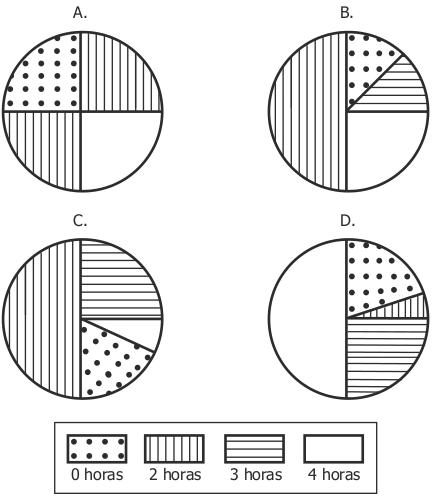
\includegraphics[scale=.5]{Images/diagramas-circulares.png}
  \question En un mapa, la distancia entre dos pueblos es 16 centímetros. La distancia real entre estos dos pueblos es de 48 kilómetros. ¿Cuántos kilómetros representa cada centímetro del mapa?

\begin{oneparchoices}
    \choice 1/4
    \choice 1/3
    \CorrectChoice 3
    \choice 4
\end{oneparchoices}
\question Para preparar cierto tipo de torta que alcanza para 10 porciones de tamaño mediano, se utilizaron 500 gramos de harina. Para preparar una torta que alcance para 20 porciones del mismo tamaño, ¿cuántas libras de harina se necesitan?

\begin{choices}
    \choice Menos de 1 libra
    \choice Exactamente 1 libra
    \CorrectChoice Exactamente 2 libras
    \choice Más de 2 libras
\end{choices}

\uplevel{En un campeonato de fútbol de un colegio participan 4 equipos (\textit{E, F, G, H}) de los cuales clasifican a la final los dos que obtengan mayor cantidad de puntos después de enfrentarse todos contra todos, una sola vez. En cada partido el equipo ganador obtiene
3 puntos y el perdedor 0 puntos; en caso de empate cada equipo obtiene 1 punto.

Los siguientes son los resultados de los 4 primeros partidos.
\begin{center}
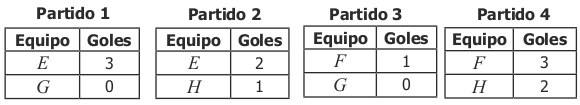
\includegraphics[scale=.4]{Images/partidos.png}
\end{center}}
\question Faltan por jugar los partidos entre los equipos \textit{E} y \textit{F} y entre los equipos \textit{G} y \textit{H}. ¿Cuál o cuáles de las siguientes afirmaciones es o son verdaderas?
\begin{itemize}
  \item[I.] \textit{E} ya está clasificado a la final.
  \item[II.] \textit{H} ya está eliminado de la final
  \item[III.] \textit{G} tiene posibilidades de clasificar a la final 
\end{itemize}
\begin{choices}
    \choice I solamente
    \CorrectChoice I y II solamente
    \choice I y III solamente.
    \choice I, II y III.
\end{choices}
\uplevel{De las siguientes afirmaciones:
\begin{itemize}
  \item[I] Todo número real tiene raíz cuadrada real
  \item[II] Los números reales negativos no tienen raíz cuadrada real
  \item[III] Los números reales negativos tienen raíz cúbica real.
\end{itemize}}
\question Sobre las anteriores afirmaciones es o son verdaderas:
\begin{choices}
    \choice I solamente
    \choice I y II
    \CorrectChoice II y III
    \choice I y III
\end{choices}
\question Al elevar un número positivo a una potencia negativa se obtiene:
\begin{choices}
    \choice Un número negativo porque $ -\times+=- $
    \choice No se puede saber
    \choice Siempre positivo y además entero.
    \CorrectChoice Un número positivo y puede ser o no un entero 
\end{choices}
  \question Al simplificar la expresión $ 2^3\times3^2\times2^4\times3^5 $ se obtiene:
\begin{choices}
    \choice $ 2^{12}\times3^{10} $ porque se multiplican los exponentes
    \CorrectChoice $ 2^7\times3^7 $ porque se suman los exponentes y se aplica la propiedad asociativa de la multiplicación
    \choice $ 2^4\times3^5 $ porque se deben dejar los exponentes mayores
    \choice $ 6^{16} $ porque se multiplican las bases y se suman los exponentes
\end{choices}
\end{multicols}
\end{questions}
%cuadro de puntajes
%\begin{center}
%\gradetable[h][pages]
%\end{center}
\end{document}